\documentclass[14pt]{extbook}
\usepackage{multicol, enumerate, enumitem, hyperref, color, soul, setspace, parskip, fancyhdr} %General Packages
\usepackage{amssymb, amsthm, amsmath, bbm, latexsym, units, mathtools} %Math Packages
\everymath{\displaystyle} %All math in Display Style
% Packages with additional options
\usepackage[headsep=0.5cm,headheight=12pt, left=1 in,right= 1 in,top= 1 in,bottom= 1 in]{geometry}
\usepackage[usenames,dvipsnames]{xcolor}
\usepackage{dashrule}  % Package to use the command below to create lines between items
\newcommand{\litem}[1]{\item#1\hspace*{-1cm}\rule{\textwidth}{0.4pt}}
\pagestyle{fancy}
\lhead{Progress Quiz 4}
\chead{}
\rhead{Version A}
\lfoot{9187-5854}
\cfoot{}
\rfoot{Spring 2021}
\begin{document}

\begin{enumerate}
\litem{
Solve the quadratic equation below. Then, choose the intervals that the solutions $x_1$ and $x_2$ belong to, with $x_1 \leq x_2$.\[ 20x^{2} -21 x -54 = 0 \]\begin{enumerate}[label=\Alph*.]
\item \( x_1 \in [-5.25, -1.96] \text{ and } x_2 \in [0.59, 1.06] \)
\item \( x_1 \in [-7.87, -5.36] \text{ and } x_2 \in [0.1, 0.54] \)
\item \( x_1 \in [-24.05, -23.74] \text{ and } x_2 \in [44.65, 45.07] \)
\item \( x_1 \in [-0.65, -0.32] \text{ and } x_2 \in [6.63, 6.8] \)
\item \( x_1 \in [-1.38, -0.7] \text{ and } x_2 \in [1.94, 2.3] \)

\end{enumerate} }
\litem{
Solve the quadratic equation below. Then, choose the intervals that the solutions belong to, with $x_1 \leq x_2$ (if they exist).\[ 17x^{2} -8 x -8 = 0 \]\begin{enumerate}[label=\Alph*.]
\item \( x_1 \in [-24.49, -23.63] \text{ and } x_2 \in [23.5, 25.3] \)
\item \( x_1 \in [-0.85, 0.67] \text{ and } x_2 \in [0.5, 1.9] \)
\item \( x_1 \in [-1.24, -0.76] \text{ and } x_2 \in [-1.6, 0.9] \)
\item \( x_1 \in [-8.7, -7.84] \text{ and } x_2 \in [15.3, 16.8] \)
\item \( \text{There are no Real solutions.} \)

\end{enumerate} }
\litem{
Write the equation of the graph presented below in the form $f(x)=ax^2+bx+c$, assuming  $a=1$ or $a=-1$. Then, choose the intervals that $a, b,$ and $c$ belong to.
\begin{center}
    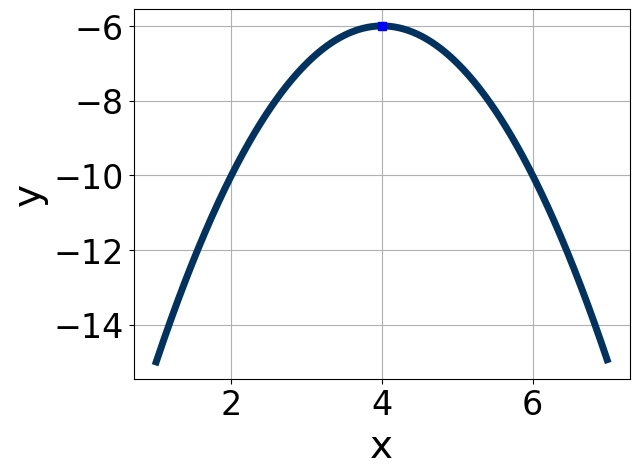
\includegraphics[width=0.5\textwidth]{../Figures/quadraticGraphToEquationA.png}
\end{center}
\begin{enumerate}[label=\Alph*.]
\item \( a \in [0.7, 1.1], \hspace*{5mm} b \in [-5, -2], \text{ and } \hspace*{5mm} c \in [7, 11] \)
\item \( a \in [-1.5, -0.3], \hspace*{5mm} b \in [2, 8], \text{ and } \hspace*{5mm} c \in [-11, -9] \)
\item \( a \in [-1.5, -0.3], \hspace*{5mm} b \in [-5, -2], \text{ and } \hspace*{5mm} c \in [2, 7] \)
\item \( a \in [-1.5, -0.3], \hspace*{5mm} b \in [2, 8], \text{ and } \hspace*{5mm} c \in [2, 7] \)
\item \( a \in [0.7, 1.1], \hspace*{5mm} b \in [2, 8], \text{ and } \hspace*{5mm} c \in [7, 11] \)

\end{enumerate} }
\litem{
Graph the equation below.\[ f(x) = (x+3)^2 + 15 \]\begin{enumerate}[label=\Alph*.]
\begin{multicols}{2}\item 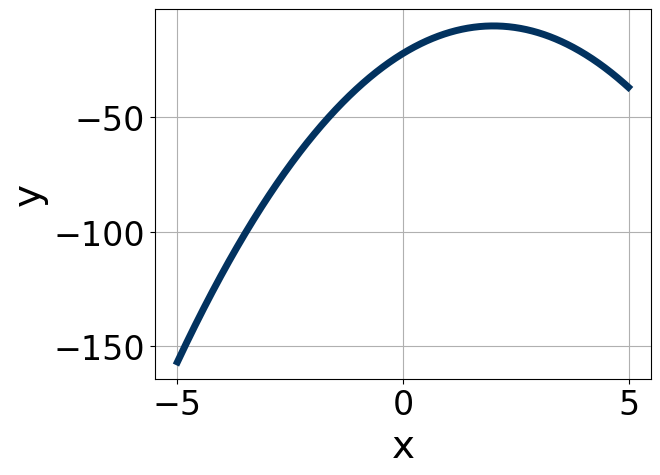
\includegraphics[width = 0.3\textwidth]{../Figures/quadraticEquationToGraphCopyAA.png}\item 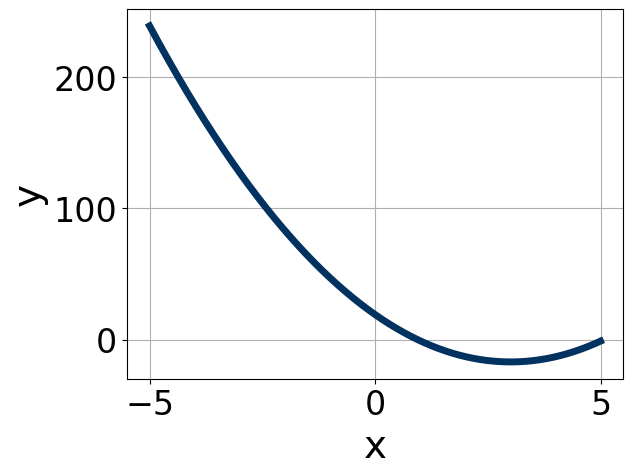
\includegraphics[width = 0.3\textwidth]{../Figures/quadraticEquationToGraphCopyBA.png}\item 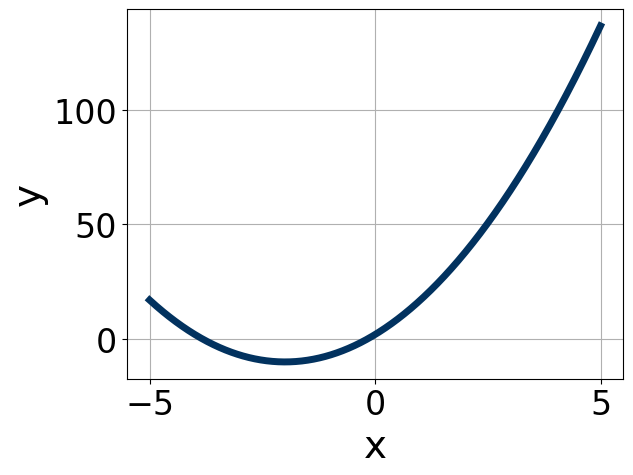
\includegraphics[width = 0.3\textwidth]{../Figures/quadraticEquationToGraphCopyCA.png}\item 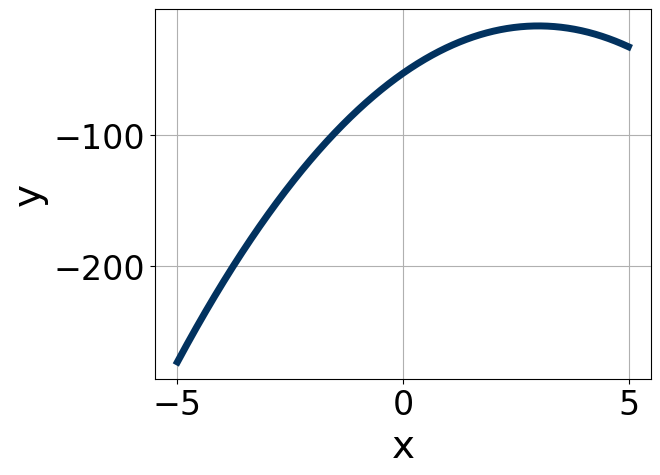
\includegraphics[width = 0.3\textwidth]{../Figures/quadraticEquationToGraphCopyDA.png}\end{multicols}\item None of the above.
\end{enumerate} }
\litem{
Write the equation of the graph presented below in the form $f(x)=ax^2+bx+c$, assuming  $a=1$ or $a=-1$. Then, choose the intervals that $a, b,$ and $c$ belong to.
\begin{center}
    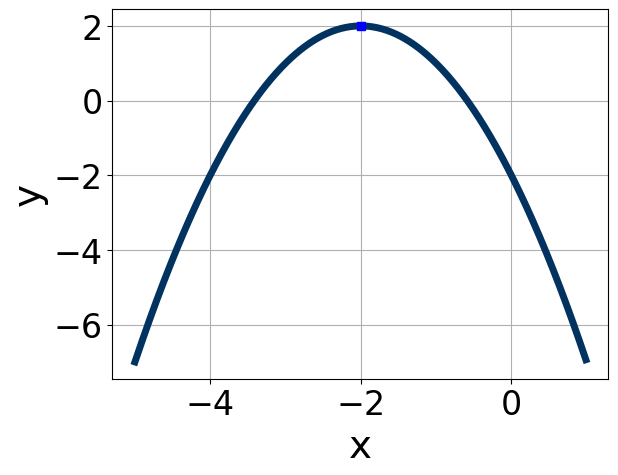
\includegraphics[width=0.5\textwidth]{../Figures/quadraticGraphToEquationCopyA.png}
\end{center}
\begin{enumerate}[label=\Alph*.]
\item \( a \in [-3, 0], \hspace*{5mm} b \in [7, 14], \text{ and } \hspace*{5mm} c \in [-15, -9] \)
\item \( a \in [1, 2], \hspace*{5mm} b \in [-11, -6], \text{ and } \hspace*{5mm} c \in [15, 21] \)
\item \( a \in [-3, 0], \hspace*{5mm} b \in [-11, -6], \text{ and } \hspace*{5mm} c \in [-15, -9] \)
\item \( a \in [1, 2], \hspace*{5mm} b \in [7, 14], \text{ and } \hspace*{5mm} c \in [15, 21] \)
\item \( a \in [-3, 0], \hspace*{5mm} b \in [-11, -6], \text{ and } \hspace*{5mm} c \in [-20, -16] \)

\end{enumerate} }
\litem{
Solve the quadratic equation below. Then, choose the intervals that the solutions belong to, with $x_1 \leq x_2$ (if they exist).\[ -20x^{2} +11 x + 2 = 0 \]\begin{enumerate}[label=\Alph*.]
\item \( x_1 \in [-13.92, -13.81] \text{ and } x_2 \in [2.68, 3.49] \)
\item \( x_1 \in [-0.43, -0.03] \text{ and } x_2 \in [0.42, 1.98] \)
\item \( x_1 \in [-16.54, -16.14] \text{ and } x_2 \in [16.71, 17.18] \)
\item \( x_1 \in [-1.26, -0.53] \text{ and } x_2 \in [-0.49, 0.67] \)
\item \( \text{There are no Real solutions.} \)

\end{enumerate} }
\litem{
Factor the quadratic below. Then, choose the intervals that contain the constants in the form $(ax+b)(cx+d); b \leq d.$\[ 54x^{2} +57 x + 10 \]\begin{enumerate}[label=\Alph*.]
\item \( a \in [1.8, 5.1], \hspace*{5mm} b \in [1, 6], \hspace*{5mm} c \in [16, 18.9], \text{ and } \hspace*{5mm} d \in [4, 9] \)
\item \( a \in [14.9, 19.3], \hspace*{5mm} b \in [1, 6], \hspace*{5mm} c \in [2.5, 3.9], \text{ and } \hspace*{5mm} d \in [4, 9] \)
\item \( a \in [7.1, 10.4], \hspace*{5mm} b \in [1, 6], \hspace*{5mm} c \in [4.5, 7.3], \text{ and } \hspace*{5mm} d \in [4, 9] \)
\item \( a \in [0, 1.9], \hspace*{5mm} b \in [10, 18], \hspace*{5mm} c \in [0.7, 1.3], \text{ and } \hspace*{5mm} d \in [43, 49] \)
\item \( \text{None of the above.} \)

\end{enumerate} }
\litem{
Solve the quadratic equation below. Then, choose the intervals that the solutions $x_1$ and $x_2$ belong to, with $x_1 \leq x_2$.\[ 25x^{2} +75 x + 54 = 0 \]\begin{enumerate}[label=\Alph*.]
\item \( x_1 \in [-45.78, -43.82] \text{ and } x_2 \in [-30.18, -29.87] \)
\item \( x_1 \in [-6.14, -4.41] \text{ and } x_2 \in [-0.47, -0.27] \)
\item \( x_1 \in [-3.99, -2.9] \text{ and } x_2 \in [-0.64, -0.5] \)
\item \( x_1 \in [-1.96, -1.31] \text{ and } x_2 \in [-1.23, -1.1] \)
\item \( x_1 \in [-9.46, -8.78] \text{ and } x_2 \in [-0.31, -0.24] \)

\end{enumerate} }
\litem{
Factor the quadratic below. Then, choose the intervals that contain the constants in the form $(ax+b)(cx+d); b \leq d.$\[ 24x^{2} +2 x -15 \]\begin{enumerate}[label=\Alph*.]
\item \( a \in [-0.3, 2.4], \hspace*{5mm} b \in [-22, -17], \hspace*{5mm} c \in [-0.9, 1.6], \text{ and } \hspace*{5mm} d \in [18, 25] \)
\item \( a \in [-0.3, 2.4], \hspace*{5mm} b \in [-6, 3], \hspace*{5mm} c \in [16.5, 20.7], \text{ and } \hspace*{5mm} d \in [5, 8] \)
\item \( a \in [1.7, 5.6], \hspace*{5mm} b \in [-6, 3], \hspace*{5mm} c \in [4.2, 9.6], \text{ and } \hspace*{5mm} d \in [5, 8] \)
\item \( a \in [7.7, 10.6], \hspace*{5mm} b \in [-6, 3], \hspace*{5mm} c \in [1.1, 3.5], \text{ and } \hspace*{5mm} d \in [5, 8] \)
\item \( \text{None of the above.} \)

\end{enumerate} }
\litem{
Graph the equation below.\[ f(x) = -(x-1)^2 - 18 \]\begin{enumerate}[label=\Alph*.]
\begin{multicols}{2}\item 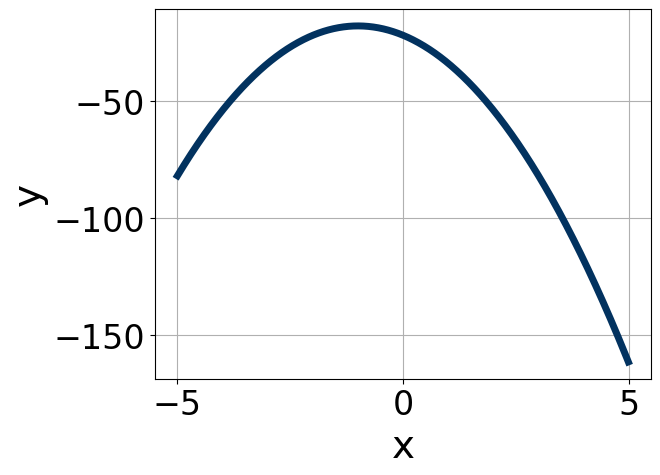
\includegraphics[width = 0.3\textwidth]{../Figures/quadraticEquationToGraphAA.png}\item 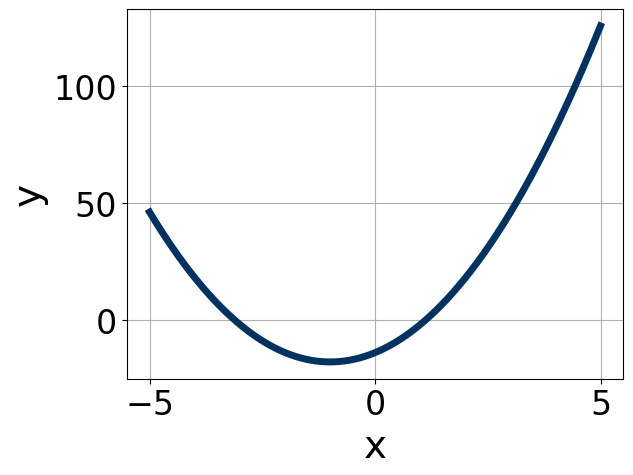
\includegraphics[width = 0.3\textwidth]{../Figures/quadraticEquationToGraphBA.png}\item 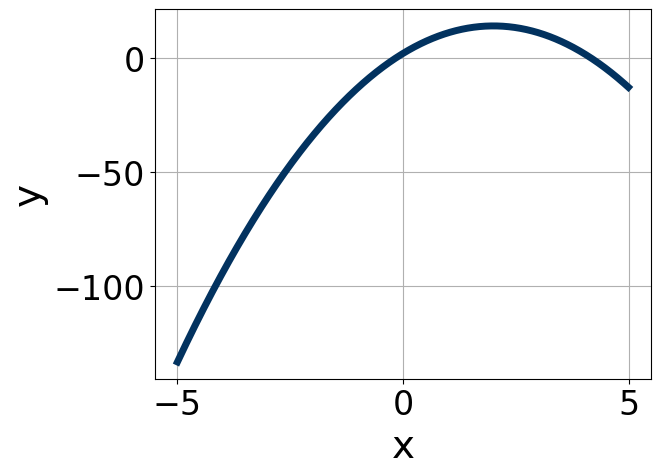
\includegraphics[width = 0.3\textwidth]{../Figures/quadraticEquationToGraphCA.png}\item 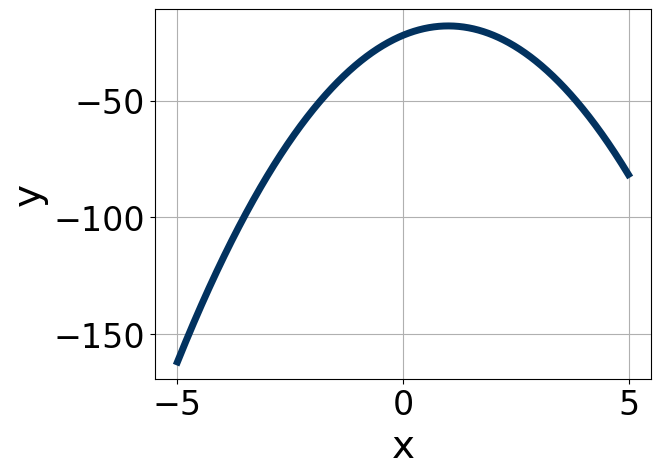
\includegraphics[width = 0.3\textwidth]{../Figures/quadraticEquationToGraphDA.png}\end{multicols}\item None of the above.
\end{enumerate} }
\end{enumerate}

\end{document}